\documentclass{article}
\usepackage[utf8]{inputenc}
\usepackage{graphicx}
\usepackage[polish]{babel}
\usepackage[T1]{fontenc}
\usepackage{longtable}
\usepackage{pgfplots}
\pgfplotsset{width=10cm,compat=1.9}

\title{sprawozdanie}
\author{Maksymilian Szewczyk}
\date{December 2022}

\begin{document}

\maketitle

\section{Wprowadzenie teoretyczne.}

Spadek swobodny to ruch, który odbywa się wyłacznie pod wpływem ciężaru, czyli siły grawitacji, bez oporów powietrza. Jego przykładem jest ruch planet wokół Słońca. Kinetyczne równanie ruchu \ref{równanie 1}:

\begin{equation}
\label{równanie 1}
    h(t) = h_0 - \frac{gt^2}{2}
\end{equation}    


gdzie h(t) to wysokość na jakiej znajduje się ciało po czasie t, 

$h_0$ to wysokość z jakiej spada ciało, a t to czas spadania.

\vspace{5mm} %5mm vertical space

źródło: https://pl.wikipedia.org/wiki/Spadek.swobodny

\section{Opis eksperymentu.}

Schemat wykonania doświadczenia przedstawiony jest na rysunku \ref{spadek.swobodny}.

\begin{figure}[htbp]
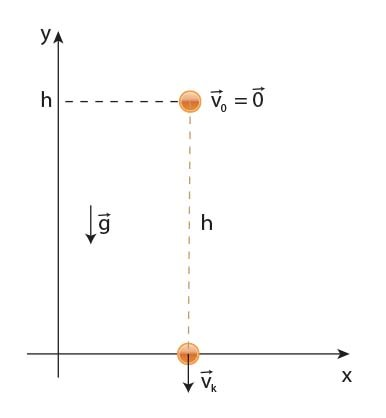
\includegraphics[width=6cm]{zdj.jpg}
\centering
\caption{Spadek swobodny.}
\label{spadek.swobodny}
\end{figure}

\vspace{5mm} %5mm vertical space
źródło: https://www.medianauka.pl/spadek-swobodny 

\section{Wyniki pomiarów}

Wyniki pomiarów przedstawione są na wykresie 1 oraz w tabeli \ref{Wyniki.pomiarów}.

\begin{tikzpicture}
\begin{axis}[
    title={Wykres spadku swobodnego},
    xlabel={t[s]},
    ylabel={s[m]},
    xmin=0, xmax=10,
    ymin=0, ymax=600,
    domain=0:10,
    xtick={0,0.7,1.4,2.1,2.8,3.5,4.2,4.9,5.6,6.3,7,7.7,8.4,9.1,9.8},
    ytick={0,50,100,150,200,250,300,350,400,450,500,550,600},
    ymajorgrids=true,
    grid style=dashed,
]
\addplot
[
    color=darkgray,
    mark=,
    mark size=20pt,
]
 {9.8 * x^2 * 0.5};

\addplot
[
    color=teal,
    only marks,
    mark=diamond,
    mark size=0.4pt
 ]
    table[meta=t]
    {csvdosprawozdania.csv};
 
\end{axis}
\end{tikzpicture}




    \centering
    \begin{longtable}{|r|r|r|}  
    \caption{Wyniki pomiarów}  
    \label{Wyniki.pomiarów}  \\
    \hline
       \bf Lp. & \bf t[s] & \bf s[m]  \\ \hline
        1 & 0,1 & 1,10 \\ 
        2 & 0,2 & 2,20 \\ 
        3 & 0,3 & 3,30 \\ 
        4 & 0,4 & 4,40 \\ 
        5 & 0,5 & 5,50 \\ 
        6 & 0,6 & 6,60 \\ 
        7 & 0,7 & 7,70 \\ 
        8 & 0,8 & 8,80 \\ 
        9 & 0,9 & 9,90 \\ 
        10 & 1,0 & 11,00 \\ 
        11 & 1,1 & 12,10 \\ 
        12 & 1,2 & 13,20 \\ 
        13 & 1,3 & 14,30 \\ 
        14 & 1,4 & 15,40 \\ 
        15 & 1,5 & 16,50 \\ 
        16 & 1,6 & 17,60 \\ 
        17 & 1,7 & 18,70 \\ 
        18 & 1,8 & 19,80 \\ 
        19 & 1,9 & 20,90 \\ 
        20 & 2,0 & 22,00 \\ 
        21 & 2,1 & 23,10 \\ 
        22 & 2,2 & 24,20 \\ 
        23 & 2,3 & 25,30 \\ 
        24 & 2,4 & 26,40 \\ 
        25 & 2,5 & 27,50 \\ 
        26 & 2,6 & 28,60 \\ 
        27 & 2,7 & 29,70 \\ 
        28 & 2,8 & 30,80 \\ 
        29 & 2,9 & 31,90 \\ 
        30 & 3,0 & 33,00 \\ 
        31 & 3,1 & 34,10 \\ 
        32 & 3,2 & 35,20 \\ 
        33 & 3,3 & 36,30 \\ 
        34 & 3,4 & 37,40 \\ 
        35 & 3,5 & 38,50 \\ 
        36 & 3,6 & 39,60 \\ 
        37 & 3,7 & 40,70 \\ 
        38 & 3,8 & 41,80 \\ 
        39 & 3,9 & 42,90 \\ 
        40 & 4,0 & 44,00 \\ 
        41 & 4,1 & 45,10 \\ 
        42 & 4,2 & 46,20 \\ 
        43 & 4,3 & 47,30 \\ 
        44 & 4,4 & 48,40 \\ 
        45 & 4,5 & 49,50 \\ 
        46 & 4,6 & 50,60 \\ 
        47 & 4,7 & 51,70 \\ 
        48 & 4,8 & 52,80 \\ 
        49 & 4,9 & 53,90 \\ 
        50 & 5,0 & 55,00 \\ 
        51 & 5,1 & 56,10 \\ 
        52 & 5,2 & 57,20 \\ 
        53 & 5,3 & 58,30 \\ 
        54 & 5,4 & 59,40 \\ 
        55 & 5,5 & 60,50 \\ 
        56 & 5,6 & 61,60 \\ 
        57 & 5,7 & 62,70 \\ 
        58 & 5,8 & 63,80 \\ 
        59 & 5,9 & 64,90 \\ 
        60 & 6,0 & 66,00 \\ 
        61 & 6,1 & 67,10 \\ 
        62 & 6,2 & 68,20 \\ 
        63 & 6,3 & 69,30 \\ 
        64 & 6,4 & 70,40 \\ 
        65 & 6,5 & 71,50 \\ 
        66 & 6,6 & 72,60 \\ 
        67 & 6,7 & 73,70 \\ 
        68 & 6,8 & 74,80 \\ 
        69 & 6,9 & 75,90 \\ 
        70 & 7,0 & 77,00 \\ 
        71 & 7,1 & 78,10 \\ 
        72 & 7,2 & 79,20 \\ 
        73 & 7,3 & 80,30 \\ 
        74 & 7,4 & 81,40 \\ 
        75 & 7,5 & 82,50 \\ 
        76 & 7,6 & 83,60 \\ 
        77 & 7,7 & 84,70 \\ 
        78 & 7,8 & 85,80 \\ 
        79 & 7,9 & 86,90 \\ 
        80 & 8,0 & 88,00 \\ 
        81 & 8,1 & 89,10 \\ 
        82 & 8,2 & 90,20 \\ 
        83 & 8,3 & 91,30 \\ 
        84 & 8,4 & 92,40 \\ 
        85 & 8,5 & 93,50 \\ 
        86 & 8,6 & 94,60 \\ 
        87 & 8,7 & 95,70 \\ 
        88 & 8,8 & 96,80 \\ 
        89 & 8,9 & 97,90 \\ 
        90 & 9,0 & 99,00 \\ 
        91 & 9,1 & 100,10 \\ 
        92 & 9,2 & 101,20 \\ 
        93 & 9,3 & 102,30 \\ 
        94 & 9,4 & 103,40 \\ 
        95 & 9,5 & 104,50 \\ 
        96 & 9,6 & 105,60 \\ 
        97 & 9,7 & 106,70 \\ 
        98 & 9,8 & 107,80 \\ 
        99 & 9,9 & 108,90 \\
        100 & 10,0 & 110,00 \\ 
        \hline
    \end{longtable}

\section{Wnioski.}

Wszystkie ciała w polu grawitacyjnym spadają z takim samym przyspieszeniem.

\end{document}
